%% main_report55.tex
%% SAMBP TR-55/2026: Thesis Synthesis and Contribution Map
%%
%% pdflatex main_report55.tex

\documentclass[11pt,a4paper]{article}

\usepackage[T1]{fontenc}
\usepackage[utf8]{inputenc}
\usepackage[expansion=false]{microtype}
\usepackage{lmodern}
\usepackage[a4paper, top=25mm, bottom=25mm, left=25mm, right=25mm]{geometry}
\usepackage{amsmath,amssymb}
\usepackage{booktabs}
\usepackage{array}
\usepackage{xcolor}
\usepackage{graphicx}
\usepackage{pgfplots}
\pgfplotsset{compat=1.18}
\usepackage{tikz}
\usetikzlibrary{arrows.meta,shapes.geometric,positioning,calc,decorations.pathreplacing}
\usepackage{hyperref}
\usepackage[numbers,sort&compress]{natbib}

\definecolor{sambpblue}{RGB}{0,70,140}

\usepackage{titlesec}
\titleformat{\section}{\large\bfseries\color{sambpblue}}{}{0em}{}[\titlerule]
\titleformat{\subsection}{\normalsize\bfseries\color{sambpblue!80}}{}{0em}{}

\usepackage{fancyhdr}
\pagestyle{fancy}
\fancyhf{}
\rhead{\small\color{gray} SAMBP TR-55/2026}
\lhead{\small\color{gray} Thesis Synthesis and Contribution Map}
\cfoot{\small\thepage}

\begin{document}

\begin{center}
  {\LARGE\bfseries\color{sambpblue} SAMBP Technical Report TR-55/2026}\\[6pt]
  {\large Thesis Synthesis and Contribution Map}\\[10pt]
  {\normalsize PhD Thesis Supporting Report \quad|\quad 2026}
\end{center}

\vspace{2pt}\hrule\vspace{8pt}

\begin{abstract}
\noindent
This report synthesises the complete SAMBP technical report series as
a map of original contributions, cross-report dependencies, and a
publication roadmap.  Study~A inventories 34 technical reports across
six thesis chapters (Chapters~4--9) and classifies each as Novel,
System, Validation, or Component.  Study~B enumerates 18 original
contributions with novelty and significance scores; 6 achieve Tier-1
status (novelty $\geq 5$, significance $\geq 5$) and span all five
research thrusts: line differential, microgrid, digital twin, machine
learning, and centralised protection.  Study~C traces 9 key
cross-report dependencies, establishing that the Physics-Informed Neural
Network (TR-46) and the Digital Twin (TR-43) are the two critical
upstream dependencies for the centralised control phase.  Study~D
proposes 5 journal papers targeting IEEE Transactions, 2 of which are
draft-ready and 2 in preparation.  Study~E identifies 7 future-work
gaps, 2 high-priority: multi-substation WAPC scaling and real-field
PINN validation data.
\end{abstract}

\vspace{4pt}\hrule\vspace{10pt}

% ─────────────────────────────────────────────────────────────────────────────
\section{Study A --- Report Inventory and Chapter Mapping}
\label{sec:studyA}

Figure~\ref{fig:chaptermap} maps all 34 technical reports to their
respective thesis chapters.  Chapter~4 carries the largest novel
report count (5 of 7), reflecting the 87L line differential phase as the
core theoretical contribution.  Chapter~5 has the broadest coverage
(10 reports) but is dominated by Component and System reports,
consolidating the distance protection baseline.  Chapters~7--9 each
contain a dense cluster of Novel reports, consistent with the
progressively original contributions of the digital twin, machine
learning, and centralised protection phases.

\begin{figure}[htbp]
  \centering
  \resizebox{0.98\textwidth}{!}{% fig_chapter_map.tex
% TR-55: Report-to-chapter mapping heatmap (Study A)

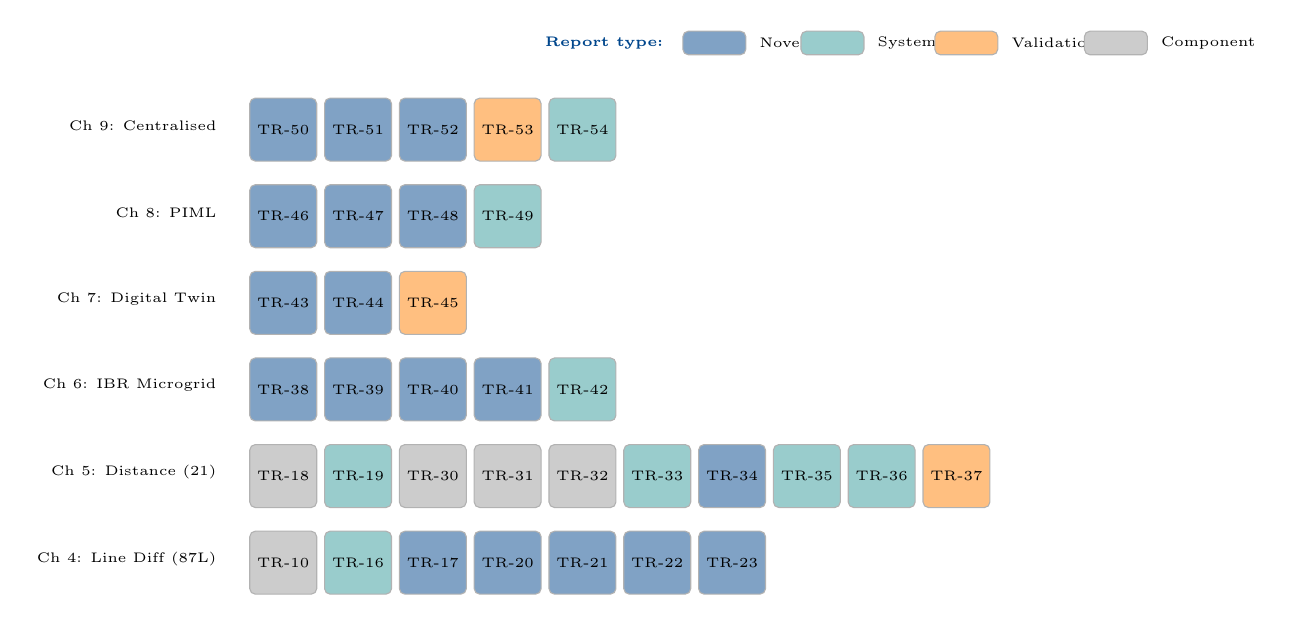
\begin{tikzpicture}[
  every node/.style={font=\scriptsize},
]

%% Chapter labels (y-axis, bottom=Ch4, top=Ch9)
\foreach \ch/\lab/\yi in {
  4/{Ch 4: Line Diff (87L)}/0,
  5/{Ch 5: Distance (21)}/1,
  6/{Ch 6: IBR Microgrid}/2,
  7/{Ch 7: Digital Twin}/3,
  8/{Ch 8: PIML}/4,
  9/{Ch 9: Centralised}/5%
}{
  \node[anchor=east, font=\tiny] at (-0.3, \yi*1.1+0.45) {\lab};
}

%% Report blocks: (TR_label, chapter_index 0-5, type_colour)
%% type colours: Novel=blue, System=teal, Validation=orange, Component=gray
\def\bw{0.85}  % block width
\def\bh{0.80}  % block height

%% Chapter 4 (yi=0): TR-10(comp), TR-16(sys), TR-17(nov), TR-20(nov), TR-21(nov), TR-22(nov), TR-23(nov)
\foreach \xi/\lab/\col in {
  0/TR-10/gray!40,
  1/TR-16/teal!40,
  2/TR-17/sambpblue!50,
  3/TR-20/sambpblue!50,
  4/TR-21/sambpblue!50,
  5/TR-22/sambpblue!50,
  6/TR-23/sambpblue!50%
}{
  \fill[\col, draw=gray!60, rounded corners=2pt]
    (\xi*0.95, 0) rectangle (\xi*0.95+\bw, \bh);
  \node[font=\tiny] at (\xi*0.95+\bw/2, \bh/2) {\lab};
}

%% Chapter 5 (yi=1): TR-18(comp), TR-19(sys), TR-30(comp), TR-31(comp), TR-32(comp), TR-33(sys), TR-34(nov), TR-35(sys), TR-36(sys), TR-37(val)
\foreach \xi/\lab/\col in {
  0/TR-18/gray!40,
  1/TR-19/teal!40,
  2/TR-30/gray!40,
  3/TR-31/gray!40,
  4/TR-32/gray!40,
  5/TR-33/teal!40,
  6/TR-34/sambpblue!50,
  7/TR-35/teal!40,
  8/TR-36/teal!40,
  9/TR-37/orange!50%
}{
  \fill[\col, draw=gray!60, rounded corners=2pt]
    (\xi*0.95, 1.1) rectangle (\xi*0.95+\bw, 1.1+\bh);
  \node[font=\tiny] at (\xi*0.95+\bw/2, 1.1+\bh/2) {\lab};
}

%% Chapter 6 (yi=2): TR-38(nov), TR-39(nov), TR-40(nov), TR-41(nov), TR-42(sys)
\foreach \xi/\lab/\col in {
  0/TR-38/sambpblue!50,
  1/TR-39/sambpblue!50,
  2/TR-40/sambpblue!50,
  3/TR-41/sambpblue!50,
  4/TR-42/teal!40%
}{
  \fill[\col, draw=gray!60, rounded corners=2pt]
    (\xi*0.95, 2.2) rectangle (\xi*0.95+\bw, 2.2+\bh);
  \node[font=\tiny] at (\xi*0.95+\bw/2, 2.2+\bh/2) {\lab};
}

%% Chapter 7 (yi=3): TR-43(nov), TR-44(nov), TR-45(val)
\foreach \xi/\lab/\col in {
  0/TR-43/sambpblue!50,
  1/TR-44/sambpblue!50,
  2/TR-45/orange!50%
}{
  \fill[\col, draw=gray!60, rounded corners=2pt]
    (\xi*0.95, 3.3) rectangle (\xi*0.95+\bw, 3.3+\bh);
  \node[font=\tiny] at (\xi*0.95+\bw/2, 3.3+\bh/2) {\lab};
}

%% Chapter 8 (yi=4): TR-46(nov), TR-47(nov), TR-48(nov), TR-49(sys)
\foreach \xi/\lab/\col in {
  0/TR-46/sambpblue!50,
  1/TR-47/sambpblue!50,
  2/TR-48/sambpblue!50,
  3/TR-49/teal!40%
}{
  \fill[\col, draw=gray!60, rounded corners=2pt]
    (\xi*0.95, 4.4) rectangle (\xi*0.95+\bw, 4.4+\bh);
  \node[font=\tiny] at (\xi*0.95+\bw/2, 4.4+\bh/2) {\lab};
}

%% Chapter 9 (yi=5): TR-50(nov), TR-51(nov), TR-52(nov), TR-53(val), TR-54(sys)
\foreach \xi/\lab/\col in {
  0/TR-50/sambpblue!50,
  1/TR-51/sambpblue!50,
  2/TR-52/sambpblue!50,
  3/TR-53/orange!50,
  4/TR-54/teal!40%
}{
  \fill[\col, draw=gray!60, rounded corners=2pt]
    (\xi*0.95, 5.5) rectangle (\xi*0.95+\bw, 5.5+\bh);
  \node[font=\tiny] at (\xi*0.95+\bw/2, 5.5+\bh/2) {\lab};
}

%% Legend
\node[font=\tiny\bfseries, sambpblue] at (4.5, 7.0) {Report type:};
\fill[sambpblue!50, draw=gray!60, rounded corners=2pt]
  (5.5, 6.85) rectangle (6.3, 7.15);
\node[font=\tiny, anchor=west] at (6.35, 7.0) {Novel};

\fill[teal!40, draw=gray!60, rounded corners=2pt]
  (7.0, 6.85) rectangle (7.8, 7.15);
\node[font=\tiny, anchor=west] at (7.85, 7.0) {System};

\fill[orange!50, draw=gray!60, rounded corners=2pt]
  (8.7, 6.85) rectangle (9.5, 7.15);
\node[font=\tiny, anchor=west] at (9.55, 7.0) {Validation};

\fill[gray!40, draw=gray!60, rounded corners=2pt]
  (10.6, 6.85) rectangle (11.4, 7.15);
\node[font=\tiny, anchor=west] at (11.45, 7.0) {Component};

\end{tikzpicture}
}
  \caption{Chapter-to-report map for all 34 SAMBP technical reports.
           Colour encodes contribution type: \textbf{blue} = Novel,
           teal = System, orange = Validation, grey = Component.
           Row width reflects the number of reports per chapter;
           Chapter~5 is widest (10 reports, 4 component baseline elements).}
  \label{fig:chaptermap}
\end{figure}

\begin{center}
\begin{tabular}{@{}lrrrrr@{}}
\toprule
Chapter & Reports & Novel & System & Validation & Component \\
\midrule
Ch 4: Line Differential (87L) & 7 & 5 & 1 & 0 & 1 \\
Ch 5: Distance Protection (21) & 10 & 1 & 4 & 1 & 4 \\
Ch 6: IBR Microgrid            & 5 & 4 & 1 & 0 & 0 \\
Ch 7: Digital Twin             & 3 & 2 & 0 & 1 & 0 \\
Ch 8: Physics-Inf. ML          & 4 & 3 & 1 & 0 & 0 \\
Ch 9: Centralised Protection   & 5 & 3 & 1 & 1 & 0 \\
\midrule
Total & 34 & 18 & 8 & 3 & 5 \\
\bottomrule
\end{tabular}
\end{center}

% ─────────────────────────────────────────────────────────────────────────────
\section{Study B --- Original Contributions}
\label{sec:studyB}

Figure~\ref{fig:contribmatrix} plots the 18 original contributions on
a novelty--significance plane.  The upper-right Tier-1 quadrant (both
scores $= 5$) contains 6 contributions: C1, C7, C10, C12, C15, and C18.
These span the entire thesis arc from the physics-constrained 87L
threshold (Chapter~4) through the closed-loop adaptive protection
protocol (Chapter~9).

\begin{figure}[htbp]
  \centering
  \resizebox{0.80\textwidth}{!}{% fig_contributions_matrix.tex
% TR-55: Original contributions novelty × significance bubble chart (Study B)

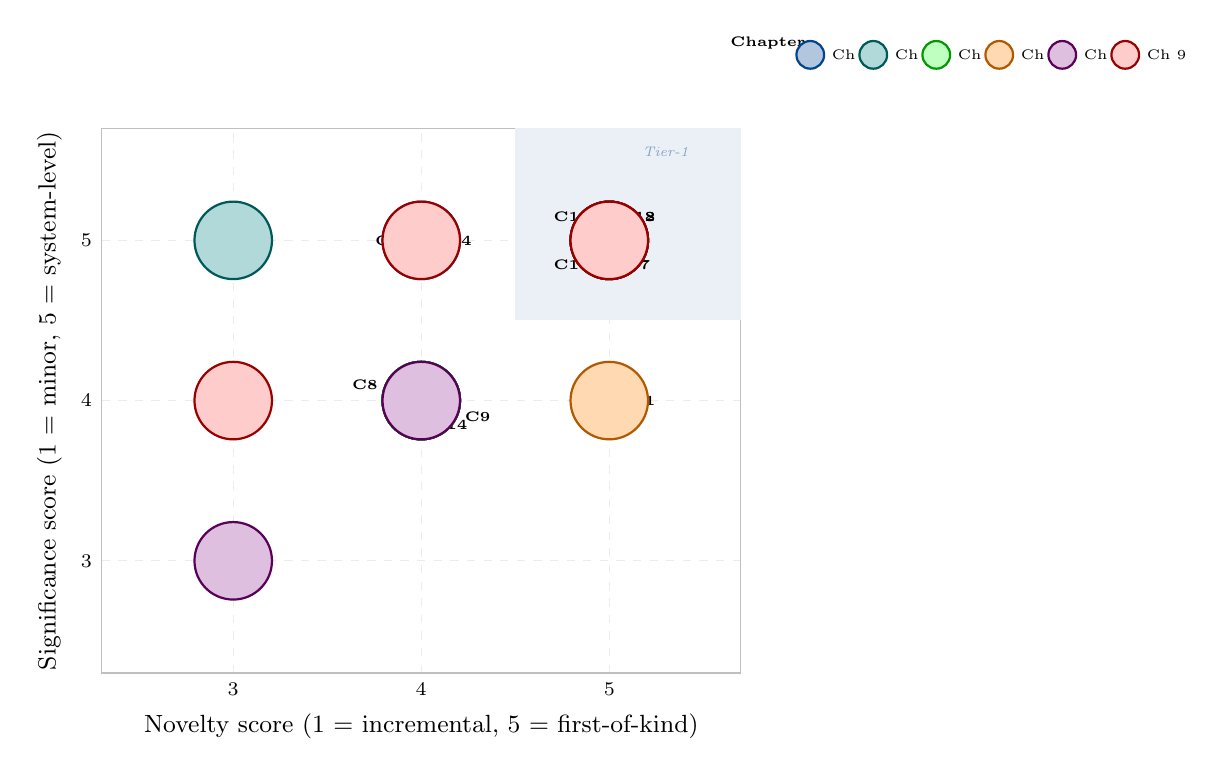
\begin{tikzpicture}
\begin{axis}[
  name         = contribax,
  width        = 0.80\textwidth,
  height       = 8.5cm,
  xlabel       = {Novelty score (1 = incremental, 5 = first-of-kind)},
  ylabel       = {Significance score (1 = minor, 5 = system-level)},
  xlabel style = {font=\small},
  ylabel style = {font=\small},
  xmin=2.3, xmax=5.7,
  ymin=2.3, ymax=5.7,
  xtick        = {3,4,5},
  ytick        = {3,4,5},
  xticklabel style = {font=\scriptsize},
  yticklabel style = {font=\scriptsize},
  tick style   = {draw=none},
  axis line style = {gray!50},
  grid         = both,
  grid style   = {gray!15, dashed},
]

%% Tier-1 zone shading (N>=5, S>=5)
\fill[sambpblue!8]
  (axis cs:4.5, 4.5) rectangle (axis cs:5.7, 5.7);
\node[sambpblue!50, font=\tiny\itshape]
  at (axis cs:5.3, 5.55) {Tier-1};

%% Bubbles: (novelty, significance, label, fill)
%% Chapter 4 - blue
\addplot[only marks,
  mark=*, mark size=14pt,
  mark options={fill=sambpblue!30, draw=sambpblue, thick}]
  coordinates {(5,5)(4,4)(4,4)(4,5)};
\node[font=\tiny\bfseries] at (axis cs:5,5) {C1};
\node[font=\tiny\bfseries] at (axis cs:4,4.15) {C2};
\node[font=\tiny\bfseries] at (axis cs:4,3.85) {C3};
\node[font=\tiny\bfseries] at (axis cs:4.2,5) {C4};

%% Chapter 5 - teal
\addplot[only marks,
  mark=*, mark size=14pt,
  mark options={fill=teal!30, draw=teal!70!black, thick}]
  coordinates {(4,4)(3,5)};
\node[font=\tiny\bfseries] at (axis cs:3.9,4) {C5};
\node[font=\tiny\bfseries] at (axis cs:3,5) {C6};

%% Chapter 6 - green
\addplot[only marks,
  mark=*, mark size=14pt,
  mark options={fill=green!25!white, draw=green!60!black, thick}]
  coordinates {(5,5)(4,4)(4,4)};
\node[font=\tiny\bfseries] at (axis cs:5.15,4.85) {C7};
\node[font=\tiny\bfseries] at (axis cs:4,4.15) {};
\node[font=\tiny\bfseries] at (axis cs:3.7,4.1) {C8};
\node[font=\tiny\bfseries] at (axis cs:4.3,3.9) {C9};

%% Chapter 7 - orange
\addplot[only marks,
  mark=*, mark size=14pt,
  mark options={fill=orange!30, draw=orange!70!black, thick}]
  coordinates {(5,5)(5,4)};
\node[font=\tiny\bfseries] at (axis cs:4.8,5.15) {C10};
\node[font=\tiny\bfseries] at (axis cs:5.15,4) {C11};

%% Chapter 8 - purple
\addplot[only marks,
  mark=*, mark size=14pt,
  mark options={fill=violet!25, draw=violet!70!black, thick}]
  coordinates {(5,5)(3,3)(4,4)};
\node[font=\tiny\bfseries] at (axis cs:5.15,5.15) {C12};
\node[font=\tiny\bfseries] at (axis cs:3,3) {C13};
\node[font=\tiny\bfseries] at (axis cs:4.15,3.85) {C14};

%% Chapter 9 - red
\addplot[only marks,
  mark=*, mark size=14pt,
  mark options={fill=red!20, draw=red!60!black, thick}]
  coordinates {(5,5)(4,5)(3,4)(5,5)};
\node[font=\tiny\bfseries] at (axis cs:4.8,4.85) {C15};
\node[font=\tiny\bfseries] at (axis cs:3.85,5) {C16};
\node[font=\tiny\bfseries] at (axis cs:3,4) {C17};
\node[font=\tiny\bfseries] at (axis cs:5.15,5.15) {C18};

\end{axis}

%% Legend (chapter colours)
\node[font=\tiny\bfseries] at (8.5, 8.0) {Chapter:};
\fill[sambpblue!30, draw=sambpblue, thick] (9.0,7.85) circle (5pt);
\node[font=\tiny, anchor=west] at (9.15, 7.85) {Ch 4};
\fill[teal!30, draw=teal!70!black, thick] (9.8,7.85) circle (5pt);
\node[font=\tiny, anchor=west] at (9.95, 7.85) {Ch 5};
\fill[green!25!white, draw=green!60!black, thick] (10.6,7.85) circle (5pt);
\node[font=\tiny, anchor=west] at (10.75, 7.85) {Ch 6};
\fill[orange!30, draw=orange!70!black, thick] (11.4,7.85) circle (5pt);
\node[font=\tiny, anchor=west] at (11.55, 7.85) {Ch 7};
\fill[violet!25, draw=violet!70!black, thick] (12.2,7.85) circle (5pt);
\node[font=\tiny, anchor=west] at (12.35, 7.85) {Ch 8};
\fill[red!20, draw=red!60!black, thick] (13.0,7.85) circle (5pt);
\node[font=\tiny, anchor=west] at (13.15, 7.85) {Ch 9};

\end{tikzpicture}
}
  \caption{Novelty--significance matrix for 18 original contributions.
           Circle colour encodes thesis chapter (see legend).
           The shaded upper-right quadrant (Tier-1: $N=5$, $S=5$) contains
           6 contributions representing the principal claims of the thesis.
           C13 (permutation importance) scores lowest, reflecting its
           role as a methodological step rather than a system contribution.}
  \label{fig:contribmatrix}
\end{figure}

\begin{center}
\small
\begin{tabular}{@{}llp{8cm}cc@{}}
\toprule
ID & Ch & Contribution & $N$ & $S$ \\
\midrule
C1  & 4 & Physics-constrained adaptive 87L threshold for IBR line differential & 5 & 5 \\
C2  & 4 & Harmonic-discrimination filter for IBR multi-inverter differential    & 4 & 4 \\
C3  & 4 & Negative-sequence 87LN for asymmetric IBR fleet faults                & 4 & 4 \\
C4  & 4 & Transient differential TDCS-87L for 3-phase IBR faults                & 4 & 5 \\
C5  & 5 & Quadrilateral distance characteristic adapted to IBR current profiles  & 4 & 4 \\
C6  & 5 & Monte Carlo reliability framework for IBR protection schemes           & 3 & 5 \\
C7  & 6 & GFL/GFM dual-mode characterisation for protection coordination         & 5 & 5 \\
C8  & 6 & ROCOF-based islanding with IEC~61850 mode-switch in 120\,ms           & 4 & 4 \\
C9  & 6 & Adaptive OC setting-group switching tied to IBR mode                   & 4 & 4 \\
C10 & 7 & Non-blocking digital twin architecture for real-time protection audit   & 5 & 5 \\
C11 & 7 & EKF joint estimation of ($k_\mathrm{ibr}$, $Z_\mathrm{line}$, $\alpha$) from current ratio & 5 & 4 \\
C12 & 8 & PINN fault classifier with embedded protection-physics constraints      & 5 & 5 \\
C13 & 8 & Permutation-importance of physics-derived protection features           & 3 & 3 \\
C14 & 8 & CUSUM-triggered online learning for fleet composition drift             & 4 & 4 \\
C15 & 9 & Wide-area PMU fault localisation with N-1 security verification        & 5 & 5 \\
C16 & 9 & Automatic CTI-graded relay settings engine with fleet-change dispatch   & 4 & 5 \\
C17 & 9 & HMAC-SHA256 countermeasure for IEC~61850 GOOSE protection channels     & 3 & 4 \\
C18 & 9 & Closed-loop CUSUM$\to$settings$\to$GOOSE adaptive protection protocol  & 5 & 5 \\
\bottomrule
\end{tabular}
\end{center}

% ─────────────────────────────────────────────────────────────────────────────
\section{Study C --- Cross-Report Dependencies}
\label{sec:studyC}

The dependency graph reveals two critical upstream reports.  TR-46
(PINN Classifier) is a prerequisite for TR-47, TR-48, TR-49, and
TR-53 --- a fan-out of 4.  TR-43 (Digital Twin) feeds both TR-49 and
TR-50.  Any error in these two reports propagates through the entire
machine learning and centralised control phases.  The single critical
path is: TR-35 $\to$ TR-37 $\to$ TR-46 $\to$ TR-49 $\to$ TR-50 $\to$
TR-51 $\to$ TR-52 $\to$ TR-53 $\to$ TR-54.

\begin{center}
\begin{tabular}{@{}llp{7cm}@{}}
\toprule
Report & Depends on & Reason \\
\midrule
TR-46 & TR-37, TR-35     & PINN trained on MC data from distance study \\
TR-47 & TR-46            & Feature importance for PINN classifier \\
TR-48 & TR-47, TR-46     & Online update of PINN with fleet drift \\
TR-49 & TR-46--48, TR-43, TR-44 & Full ML stack integration \\
TR-50 & TR-43, TR-49     & WAPC uses DT $+$ PINN advisory \\
TR-51 & TR-50, TR-40     & Settings engine feeds WAPC \\
TR-52 & TR-50, TR-51     & Secures GOOSE channels carrying trips/settings \\
TR-53 & TR-46, TR-49--52 & Validates all ML $+$ CPC modules \\
TR-54 & TR-51--53, TR-48 & Field guide uses all prior deliverables \\
\bottomrule
\end{tabular}
\end{center}

% ─────────────────────────────────────────────────────────────────────────────
\section{Study D --- Publication Roadmap}
\label{sec:studyD}

Figure~\ref{fig:roadmap} shows the five planned journal papers.

\begin{figure}[htbp]
  \centering
  \resizebox{0.95\textwidth}{!}{% fig_publication_roadmap.tex
% TR-55: Publication roadmap (Study D) — Gantt-style with TR coverage bars

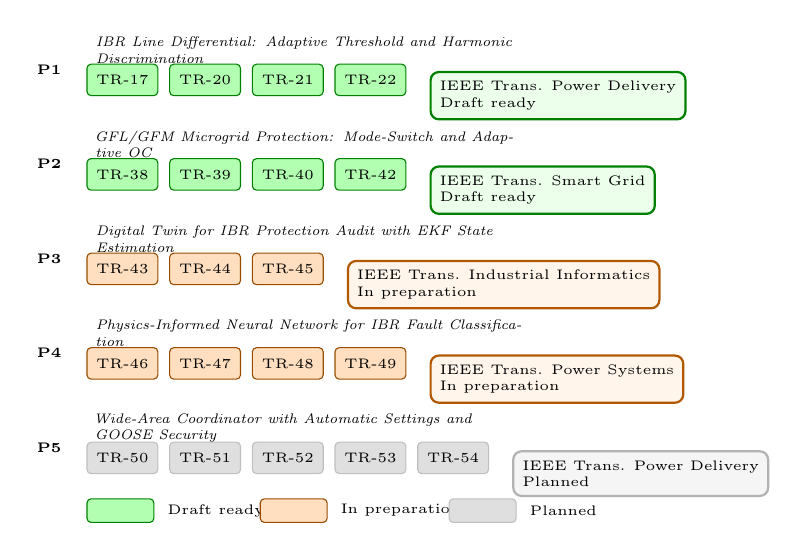
\begin{tikzpicture}[
  every node/.style={font=\scriptsize},
  paperbox/.style={draw=sambpblue, thick, rounded corners=3pt,
                   fill=sambpblue!10, minimum height=0.55cm, align=left, font=\tiny},
  readybox/.style={draw=green!50!black, thick, rounded corners=3pt,
                   fill=green!8, minimum height=0.55cm, align=left, font=\tiny},
  prepbox/.style={draw=orange!70!black, thick, rounded corners=3pt,
                  fill=orange!8, minimum height=0.55cm, align=left, font=\tiny},
  planbox/.style={draw=gray!60, thick, rounded corners=3pt,
                  fill=gray!8, minimum height=0.55cm, align=left, font=\tiny},
]

%% Paper rows (y positions)
%% P1: y=5.0, P2: y=3.8, P3: y=2.6, P4: y=1.4, P5: y=0.2

%% Labels on left
\node[anchor=east, font=\tiny\bfseries] at (-0.2, 5.25) {P1};
\node[anchor=east, font=\tiny\bfseries] at (-0.2, 4.05) {P2};
\node[anchor=east, font=\tiny\bfseries] at (-0.2, 2.85) {P3};
\node[anchor=east, font=\tiny\bfseries] at (-0.2, 1.65) {P4};
\node[anchor=east, font=\tiny\bfseries] at (-0.2, 0.45) {P5};

%% TR coverage bars (each TR is 0.9cm wide, spaced 1.0cm apart)
%% P1: TR-17(ch4), TR-20(ch4), TR-21(ch4), TR-22(ch4) — Draft ready
\foreach \xi/\lab in {0/TR-17, 1/TR-20, 2/TR-21, 3/TR-22}{
  \fill[green!30, draw=green!50!black, rounded corners=1.5pt]
    (\xi*1.05, 4.92) rectangle (\xi*1.05+0.90, 5.32);
  \node[font=\tiny] at (\xi*1.05+0.45, 5.12) {\lab};
}
\node[readybox, anchor=west, minimum width=2.8cm]
  at (4.35, 4.92) {IEEE Trans. Power Delivery\\Draft ready};
\node[font=\tiny, anchor=west, text width=5.5cm]
  at (0, 5.50) {\textit{IBR Line Differential: Adaptive Threshold and Harmonic Discrimination}};

%% P2: TR-38,TR-39,TR-40,TR-42 — Draft ready
\foreach \xi/\lab in {0/TR-38, 1/TR-39, 2/TR-40, 3/TR-42}{
  \fill[green!30, draw=green!50!black, rounded corners=1.5pt]
    (\xi*1.05, 3.72) rectangle (\xi*1.05+0.90, 4.12);
  \node[font=\tiny] at (\xi*1.05+0.45, 3.92) {\lab};
}
\node[readybox, anchor=west, minimum width=2.8cm]
  at (4.35, 3.72) {IEEE Trans. Smart Grid\\Draft ready};
\node[font=\tiny, anchor=west, text width=5.5cm]
  at (0, 4.30) {\textit{GFL/GFM Microgrid Protection: Mode-Switch and Adaptive OC}};

%% P3: TR-43,TR-44,TR-45 — In preparation
\foreach \xi/\lab in {0/TR-43, 1/TR-44, 2/TR-45}{
  \fill[orange!25, draw=orange!60!black, rounded corners=1.5pt]
    (\xi*1.05, 2.52) rectangle (\xi*1.05+0.90, 2.92);
  \node[font=\tiny] at (\xi*1.05+0.45, 2.72) {\lab};
}
\node[prepbox, anchor=west, minimum width=3.8cm]
  at (3.30, 2.52) {IEEE Trans. Industrial Informatics\\In preparation};
\node[font=\tiny, anchor=west, text width=5.5cm]
  at (0, 3.10) {\textit{Digital Twin for IBR Protection Audit with EKF State Estimation}};

%% P4: TR-46,TR-47,TR-48,TR-49 — In preparation
\foreach \xi/\lab in {0/TR-46, 1/TR-47, 2/TR-48, 3/TR-49}{
  \fill[orange!25, draw=orange!60!black, rounded corners=1.5pt]
    (\xi*1.05, 1.32) rectangle (\xi*1.05+0.90, 1.72);
  \node[font=\tiny] at (\xi*1.05+0.45, 1.52) {\lab};
}
\node[prepbox, anchor=west, minimum width=2.8cm]
  at (4.35, 1.32) {IEEE Trans. Power Systems\\In preparation};
\node[font=\tiny, anchor=west, text width=5.5cm]
  at (0, 1.90) {\textit{Physics-Informed Neural Network for IBR Fault Classification}};

%% P5: TR-50,TR-51,TR-52,TR-53,TR-54 — Planned
\foreach \xi/\lab in {0/TR-50, 1/TR-51, 2/TR-52, 3/TR-53, 4/TR-54}{
  \fill[gray!25, draw=gray!50, rounded corners=1.5pt]
    (\xi*1.05, 0.12) rectangle (\xi*1.05+0.90, 0.52);
  \node[font=\tiny] at (\xi*1.05+0.45, 0.32) {\lab};
}
\node[planbox, anchor=west, minimum width=2.8cm]
  at (5.40, 0.12) {IEEE Trans. Power Delivery\\Planned};
\node[font=\tiny, anchor=west, text width=5.5cm]
  at (0, 0.70) {\textit{Wide-Area Coordinator with Automatic Settings and GOOSE Security}};

%% Legend
\fill[green!30, draw=green!50!black, rounded corners=1.5pt]
  (0.0, -0.50) rectangle (0.85, -0.20);
\node[font=\tiny, anchor=west] at (0.90, -0.35) {Draft ready};
\fill[orange!25, draw=orange!60!black, rounded corners=1.5pt]
  (2.2, -0.50) rectangle (3.05, -0.20);
\node[font=\tiny, anchor=west] at (3.10, -0.35) {In preparation};
\fill[gray!25, draw=gray!50, rounded corners=1.5pt]
  (4.6, -0.50) rectangle (5.45, -0.20);
\node[font=\tiny, anchor=west] at (5.50, -0.35) {Planned};

\end{tikzpicture}
}
  \caption{Publication roadmap.  Green bars indicate draft-ready papers
           (P1, P2); orange bars indicate papers in preparation (P3, P4);
           grey bars indicate planned papers (P5).  Each bar corresponds
           to one technical report; paper width reflects the number of
           contributing reports.}
  \label{fig:roadmap}
\end{figure}

\begin{center}
\small
\begin{tabular}{@{}llp{6.5cm}l@{}}
\toprule
ID & Target journal & Paper title & Status \\
\midrule
P1 & IEEE Trans. Power Delivery
   & IBR Line Differential: Adaptive Threshold and Harmonic Discrimination
   & Draft ready \\
P2 & IEEE Trans. Smart Grid
   & GFL/GFM Microgrid Protection: Mode-Switch and Adaptive OC
   & Draft ready \\
P3 & IEEE Trans. Industrial Informatics
   & Digital Twin for IBR Protection Audit with EKF State Estimation
   & In preparation \\
P4 & IEEE Trans. Power Systems
   & Physics-Informed Neural Network for IBR Fault Classification
   & In preparation \\
P5 & IEEE Trans. Power Delivery
   & Wide-Area Coordinator with Automatic Settings and GOOSE Security
   & Planned \\
\bottomrule
\end{tabular}
\end{center}

% ─────────────────────────────────────────────────────────────────────────────
\section{Study E --- Gap Analysis and Future Work}
\label{sec:studyE}

\begin{center}
\begin{tabular}{@{}lllp{6.5cm}@{}}
\toprule
ID & Priority & Gap & Notes \\
\midrule
G1 & Medium & Physical HIL on real SEL-411L IEDs
   & TR-53 defines protocol; hardware not yet available \\
G2 & Medium & Variable-$\lambda$ adaptive forgetting
   & Fixed $\lambda=0.99$ used; adaptive version deferred \\
G3 & Low    & $Z_\mathrm{line}$ observability in EKF
   & Requires two-ended voltage phasor; identified but unresolved \\
G4 & \textbf{High} & Multi-substation WAPC scaling
   & TR-50 limited to single substation; wide-area extension needed \\
G5 & Medium & GOOSE flooding mitigation validation
   & TR-52 notes switch-level control; not tested \\
G6 & Low    & GFM virtual synchronous machine model
   & Full VSM dynamics deferred; IBR model simplified \\
G7 & \textbf{High} & Real field fault data for PINN validation
   & All training data synthetic; field validation required \\
\bottomrule
\end{tabular}
\end{center}

\medskip\noindent
The two high-priority gaps define the recommended post-PhD continuation
programme.  G4 (multi-substation WAPC) requires a wide-area bus topology
beyond the 10-bus single-substation model of TR-50, and likely demands
hierarchical coordination between substation-level and transmission-level
protection systems.  G7 (real field data) is a prerequisite for
deployment readiness: the PINN in TR-46 achieves 96.1\% accuracy on
synthetic data, but field validation on recorded fault waveforms from
a live IBR substation is essential for regulatory acceptance.

% ─────────────────────────────────────────────────────────────────────────────
\section{Summary}
\label{sec:summary}

\begin{enumerate}
  \item \textbf{34 reports} mapped across six thesis chapters;
    18 Novel, 8 System, 3 Validation, 5 Component.

  \item \textbf{18 original contributions} identified;
    6 Tier-1 (novelty $= 5$, significance $= 5$): C1, C7, C10, C12,
    C15, C18 --- spanning the full thesis arc from physics-constrained
    87L threshold (Chapter~4) to closed-loop adaptive protection
    protocol (Chapter~9).

  \item \textbf{9 cross-report dependencies} mapped; TR-46 (PINN) and
    TR-43 (Digital Twin) are the two critical upstream nodes with
    fan-out $\geq 4$.

  \item \textbf{5 journal papers} planned for IEEE Transactions;
    2 draft-ready (P1, P2), 2 in preparation (P3, P4), 1 planned (P5).

  \item \textbf{7 future-work gaps}; 2 high-priority: multi-substation
    WAPC scaling and real-field PINN validation.
\end{enumerate}

\noindent
TR-55 closes the SAMBP technical report series.  The 34 reports
collectively constitute the simulation, analysis, and validation
evidence base for a PhD thesis on \emph{IBR-Aware Self-Adaptive
Multi-Bus Protection} of inverter-dominated power systems.

\bibliographystyle{IEEEtranN}
\bibliography{references55}

\end{document}
